\chapter{Grundlagen der Ortung}
\label{chap2:Grundlagen}

Es existieren einige Methoden einen Punkt im Raum zu lokalisieren. Meistens werden jedoch die folgen drei angewendet: Triangulation, Fingerabdruckverfahren und Trilateration. Die Triangulation basiert auf den Trigonometrischen Funktionen. Dabei wird ein Dreieck zwischen zwei Referenzstandorten und dem gesuchten Objekt gespannt. Um dieses Dreieck eindeutig zu bestimmen, benötigt man den Abstand der beiden Referenzpunkte zueinander und die beiden Winkel der Geraden vom Objekt zum jeweiligen Referenzort. Um eine Ortung mittels Triangulation durchzuführen, sind Richtungsmessungen, \gls{AoA} an den Basistationen notwendig.

Eine zweite Möglichkeit ist das Fingerabdruckverfahren \emph{(Fingerprinting)}. Dabei wird für eine Position ein charakteristisches Merkmal in einer Datenbank gespeichert. Wird beim Messvorgang dieses Merkmal erkannt, kann es wieder der jeweiligen Position zugeordnet werden. Wichtig bei dieser Methode ist es, einzigartige Merkmale zu finden, damit zwei Positionen nicht miteinander verwechselt werden. Die beiden bisher genannten Methoden werden ebenfalls im Rahmen des \glslink{BATS}{BATS} Projektes  untersucht und von anderen Arbeiten am Lehrstuhl behandelt. 
Diese Arbeit beschäftigt sich mit der Methode der Trilateration, welche in Abbildung \ref{fig:Trilateration} veranschaulicht wird. Um die Position eines Objektes zu bestimmen, wird hierbei die Distanz zum Objekt von drei oder mehr Referenzpunkten aus geschätzt. Zieht man um die jeweiligen Referenzpunkte einen Kreis, mit der zugehörigen Distanz als Radius, findet man in deren Schnittpunkt das gesuchte Objekt.

\begin{figure}[htbp]
 \centering
 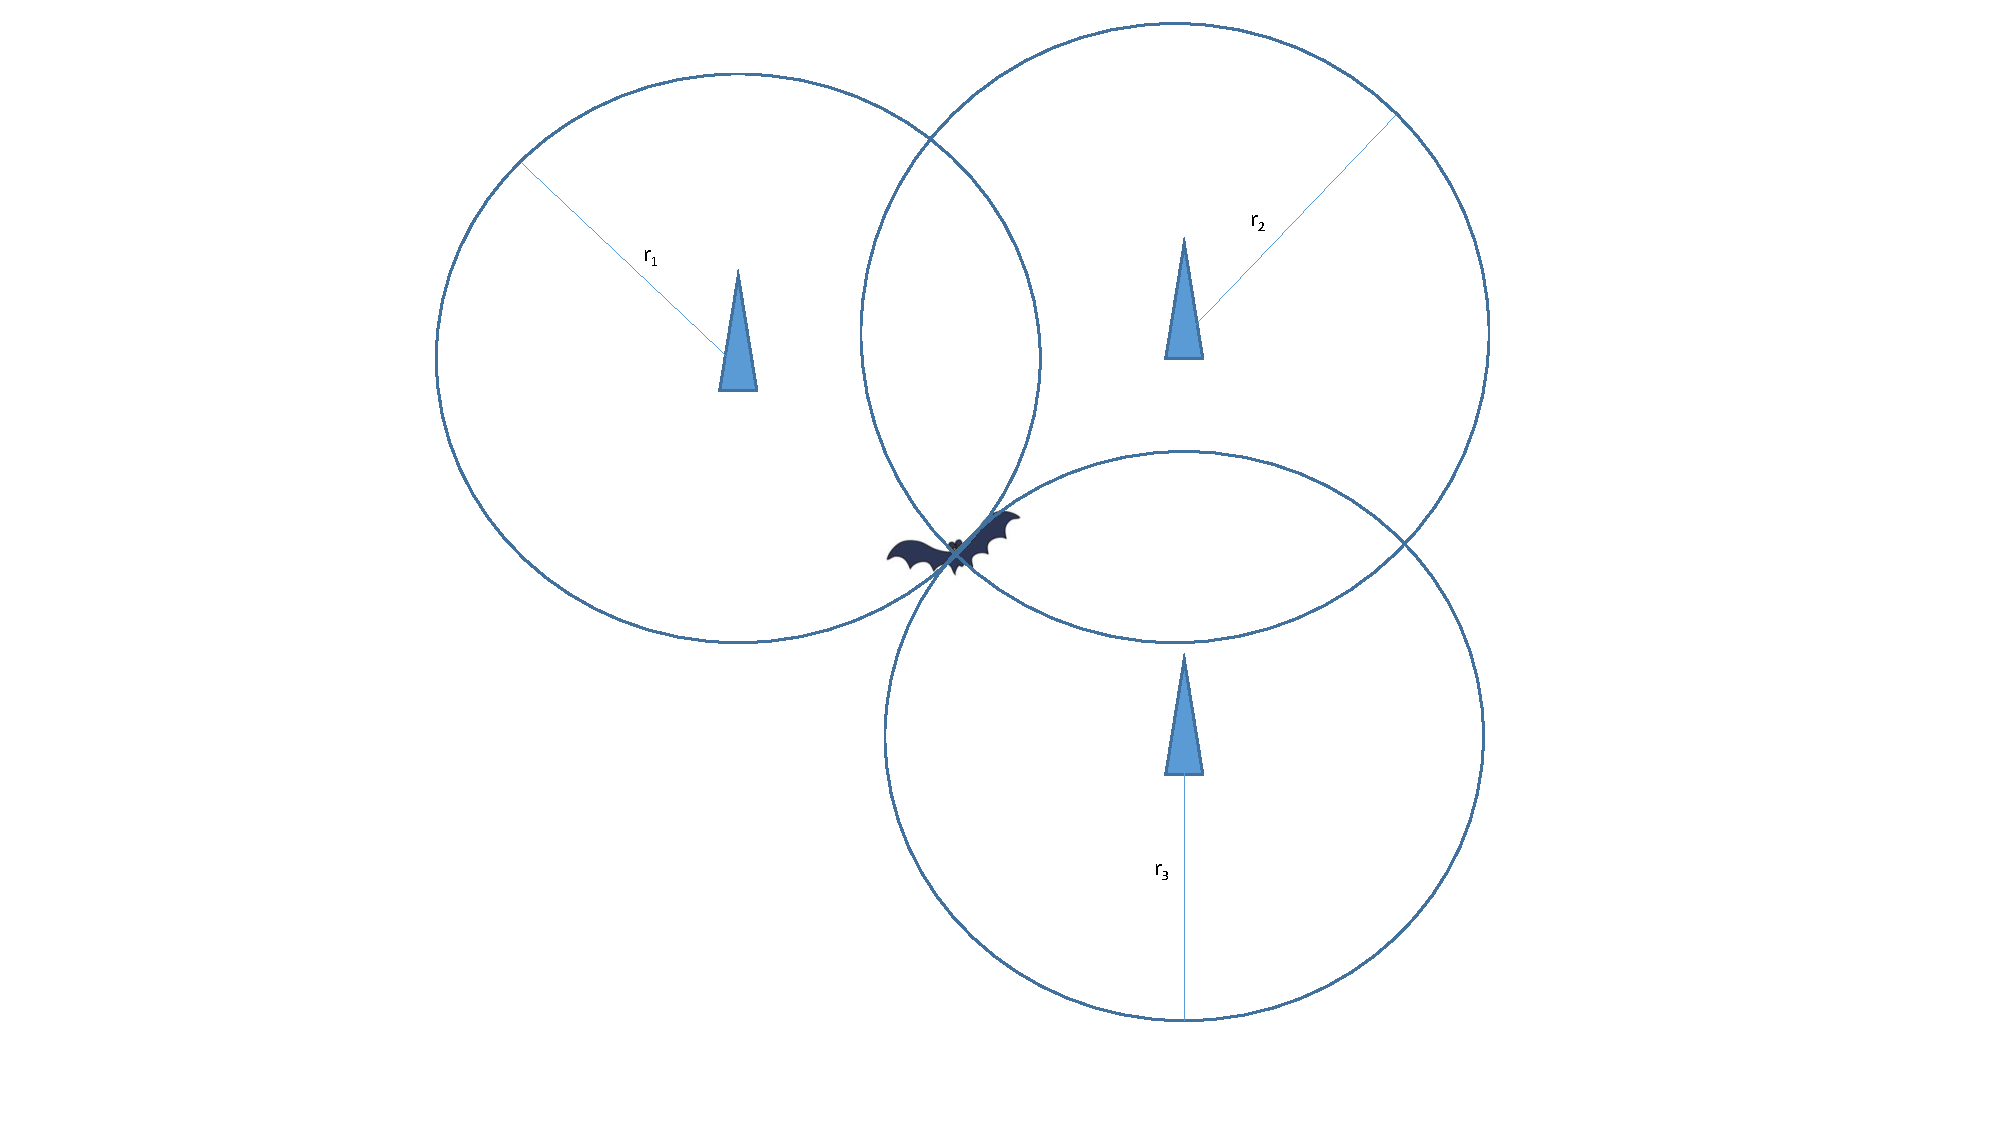
\includegraphics[width = \textwidth]{images/Trilateration}
 \caption{Trilateration}
 \label{fig:Trilateration}
\end{figure}

Ob mit dieser Methode eine hohe Genauigkeit erzielt wird, hängt davon ab, wie fehlerbehaftet die Distanzmessungen sind. Die Distanz lässt sich aus zwei unterschiedlichen Messungen gewinnen. Zum einen kann man die Signalleistung, zum anderen die Laufzeit auswerten. 
Mit Kenntnissen der Ausbreitungsdämpfung und der Sendesignalleistung ist es möglich, auf eine Distanz, die die Welle zurückgelegt haben muss, zu schließen. 

Mithilfe der Laufzeit \gls{symb:tau} und Ausbreitungsgeschwindigkeit \gls{symb:c0}\footnote{Die Ausbreitungsgeschwindigkeit einer elektromagnetischen Welle, entspricht im Vakuum der Lichtgeschwindigkeit, ist sonst aber materialabhängig.} einer elektromagnetischen Welle, ist es ebenfalls möglich die Distanz zu berechnen.

\begin{equation}
	\label{eq:Distanzberechnung}
	r = c_0\cdot \tau
\end{equation}

Die Schwierigkeit besteht darin, die Laufzeit, über einen stark gestörten Kanal, möglichst genau zu ermitteln. 

\section{Laufzeitschätzung}
\label{chap2.1:Laufzeitschätzung}
Möglichkeiten zur Ermittlung der Laufzeit beruhen auf den Ausbreitungsgesetzen elektromagnetischer Wellen. Diese lassen sich aus den Maxwell-Gleichungen, welche die Eigenschaften elektromagnetischer Felder und deren Ausbreitung beschreiben, ableiten.
Die Bestimmung der Laufzeit einer Welle, lässt sich jedoch auch Systemtheoretisch ausdrücken. Die räumliche Ausbreitung der Welle wird dabei als zeitliche Verzögerung eines Signals betrachtet. Dabei korrespondiert eine Verzögerung im Zeitbereich mit einer Phasenmodulation im Frequenzbereich. Der Verschiebungssatz der Fouriertransformation zeigt diesen Zusammenhang: 

\begin{equation}
	\label{eq:Verschiebungssatz}
	x(t - \tau) \; \laplace\; X(f)e^{-j2 \pi f_c \tau}
\end{equation}


Wenn die Trägerfrequenz \gls{symb:fc} und die Phasendrehung $\gls{symb:phi}=2\pi  \gls{symb:fc}\gls{symb:tau}$ bekannt sind, kann die Verzögerung \gls{symb:tau} bestimmt werden. 
Da die Phasendrehung aber periodisch mit der Periode $2\pi$ ist, kann keine eindeutige Aussage über die Laufzeit getroffen werden. Um das an einem Zahlenbeispiel zu verdeutlichen, soll von einem Signal mit der Frequenz \unit[1]{GHz} ausgegangen werden. Dieses Signal hat eine Periodendauer von \unit[1]{ps}. Nach \eqref{eq:Distanzberechnung} entspricht das einer Strecke von \unit[30]{cm}. Nach diesen \unit[30]{cm} wiederholt sich die Phase. Damit kann die zurückgelegte Strecke nur auf den ersten \unit[30]{cm} eindeutig bestimmt werden, da man danach nicht genau sagen kann, in welcher Periode man sich befindet. Damit ist der Eindeutigkeitsbereich der Phaseninformation der Welle auf einen Bereich von \unit[30]{cm} beschränkt. Je höher die Frequenz, desto kleiner ist der Eindeutigkeitsbereich. Dieser Bereich kann jedoch vergrößert werden, indem Phasendifferenzen verwendet werden. Dazu werden Signale mit mehreren Frequenzanteilen, sogenannte Subträger, erzeugt. Die Geschwindigkeit, mit der sich die Phase dreht, wird mit dem Phasenmaß \gls{symb:beta} $= \omega \sqrt{\epsilon \mu}$ angegeben, wobei \gls{symb:omega} der Kreisfrequenz und \gls{symb:epsilon} und \gls{symb:mu} den Materialeigenschaften entsprechen. Aus diesem Zusammenhang ist erkennbar: je höher die Frequenz, desto schneller dreht sich die Phase. Die hieraus resultierende Phasendifferenz \gls{symb:dphi} zwischen den, bei unterschiedlichen Frequenzen liegenden Subträgern, wird zur Laufzeitbestimmung verwendet. 
Je länger die Welle wandert, desto größer wird die Differenz, aufgrund der unterschiedlichen Drehgeschwindigkeiten. Allerdings ist auch der Eindeutigkeitsbereich dieser Methode begrenzt, da die Phasendifferenz selbst periodisch ist. Die Länge der Periodendauer ist vom Abstand der Subträger zueinander abhängig. Bei einem großen Abstand erfolgt die Verdrehung zueinander schneller und führt damit zu einer kürzeren Periodendauer. Somit verhält sich der Eindeutigkeitsbereich $\gls{symb:tau}_{max}$ umgekehrt proportional zum Frequenzabstand \gls{symb:df}.

\begin{equation}
	\label{eq:Eindeutigkeitsbereich}
	\tau_{max} = \frac{1}{\Delta f}
\end{equation} 

Wenn man das zuvor genannte Beispiel wieder heranzieht, und von einer Mittenfrequenz bei \unit[1]{GHz} und einer Bandbreite von \unit[2]{MHz} ausgeht, ist der größtmögliche Subträgerabstand \gls{symb:df} gleich der Bandbreite. Als kleinstmöglichen Eindeutigkeitsbereich ergeben sich \unit[150]{m}. 
Für die Laufzeitbestimmung muss die gemessene Phasendifferenz in Bezug zum jeweiligen Subträgerabstand gestellt werden, da der Abstand maßgeblich für die Stärke der Verdrehung verantwortlich ist.
Aus diesem Zusammenhängen, und aus den Gleichungen \eqref{eq:Distanzberechnung} und  \eqref{eq:Verschiebungssatz}, folgt für die Distanzschätzung mittels Phasendifferenzen folgende Beziehung \citep{nowak2014system}:

\begin{equation}
	\label{eq:Phasendifferenz}
	r = \frac{c_0}{2\pi}\cdot\frac{\partial\varphi}{\partial f}
\end{equation}

Die Ableitung der Phase nach der Frequenz entspricht einer Gruppenlaufzeit. Diese beschreibt wie lange eine Wellengruppe (mehrere Subträger) gewandert ist. 


\section{Kanalmodell}
\label{chap2.2:Kanalmodell}
Wenn die Phasen exakt gemessen werden können, ermöglicht dies eine sehr genaue Bestimmung der Laufzeit im Eindeutigkeitsbereich. Beim Detektieren von Signalen passieren jedoch häufig Fehler. Diese entstehen aufgrund von Störeinflüssen der Umgebung. Damit der Einfluss dieser Fehlerquellen verringert werden kann, muss der Übertragungskanal genauer untersucht werden. Wenn das Übertragungsverhalten des Kanals bekannt ist, können anschließend Signale und Schätzverfahren entworfen werden, um Störeinflüsse zu minimieren.   
Um Einflüsse der Umgebung zu simulieren, wird ein mathematisches Modell benötigt, welches diese beschreibt. Dabei werden die unterschiedlichen Störungen getrennt betrachtet und am Ende zusammengeführt. Die Laufzeit der Welle wird als Verzögerungsglied modelliert, welches die Phasendrehung realisieren soll.

\subsection{Additiv White Gaussian Noise (AWGN) - Kanal}
\label{chap2.2.1:AWGN}
Zunächst kann von einem \gls{AWGN}-Kanal, wie in Abbildung \ref{fig: AWGN-Kanal} ausgegangen werden. Ein solches Rauschmodell, stellt den "`\emph{worst case}"' dar, da das gesamte Band konstant verrauscht ist. Dieser Kanal addiert auf das verzögerte Sendesignal $s(t-\tau)$ eine Musterfunktion $n(t)$ aus einem Gaußschen Rauschprozess $N$ mit einem konstanten Leistungsdichtespektrum $\Phi(f) = \frac{N_0}{2}$, sodass das Empfangssignal $r(t)$ resultiert. Eine Musterfunktion entspricht einer konkreten Realisierung eines Zufallsprozesses. 

\begin{figure}[htbp]
\centering
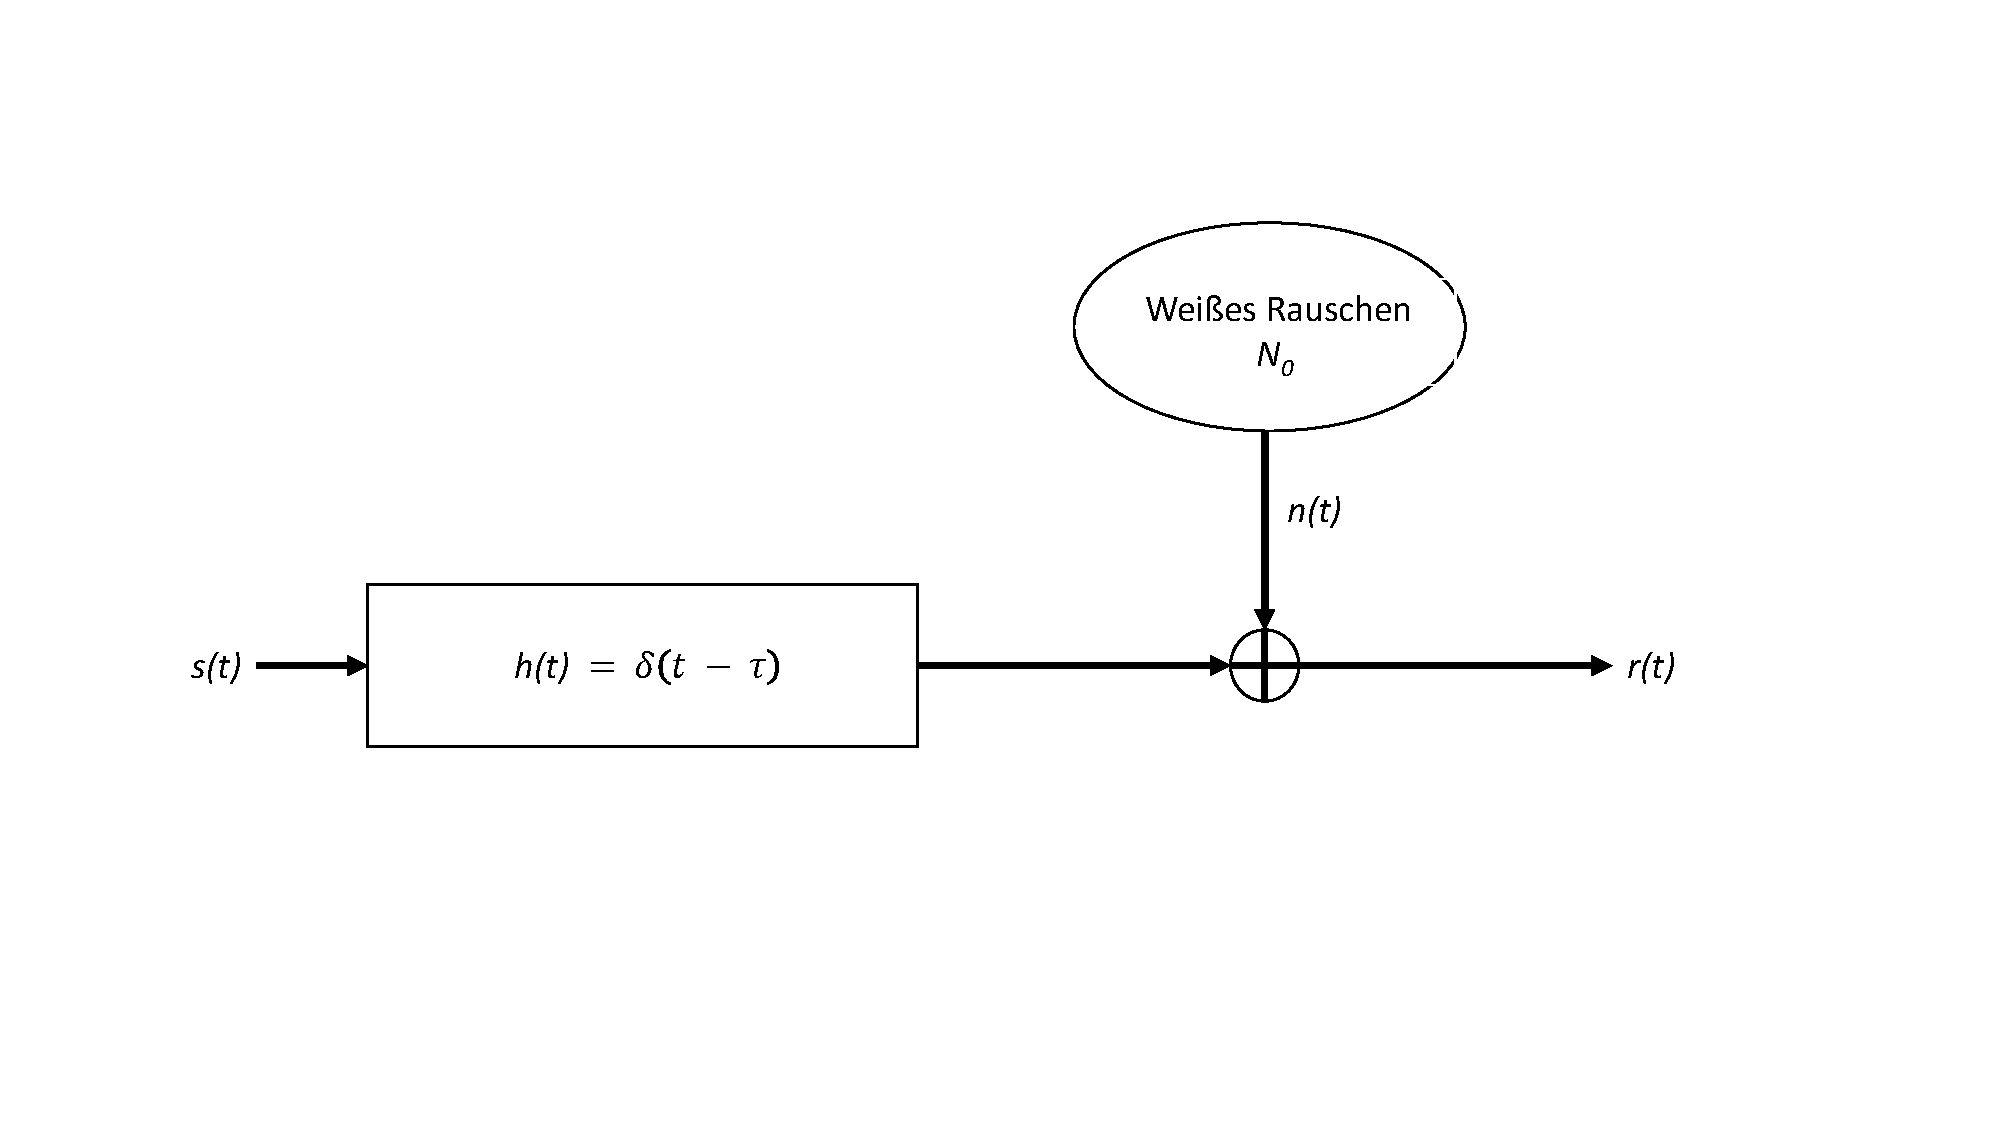
\includegraphics[width = \textwidth]{images/WeisesRauschen}
\caption{Blockschaltbild zu einem AWGN-Kanal}
\label{fig: AWGN-Kanal}
\end{figure}

Wie im vorherigen Kapitel bereits angesprochen, führt das Verzögerungsglied zu einer frequenzabhängigen Phasendrehung. Für eine feste Laufzeit ergibt sich, aufgrund des linearen Zusammenhangs zwischen Phasendrehung und Laufzeit aus \eqref{eq:Verschiebungssatz}, eine Rampe mit der Steigung $2\pi\tau$. Vernachlässigt man die Dämpfung, ist der Betragsgang der Übertragungsfunktion $H(f)$ konstant gleich eins. Die Aufgabe, der in dieser Arbeit vorgestellten Schätzverfahren, ist es, die Steigung der Phasenrampe zu ermitteln. Deshalb ist von großem Interesse, welchen Einfluss der \gls{AWGN}-Kanal auf den Phasengang des Verzögerungsgliedes hat.  In Abbildung \ref{fig: AWGN-Plot}, wurde ein solcher Kanal simuliert. Auf der rechten Seite ist der Phasengang und auf der Linken der Betragsgang eines solchen Kanals zu sehen. Durch additives Rauschen ist der Phasengang ebenfalls verrauscht, wobei es vom Signal-Rausch-Verhältnis (\gls{SNR}) abhängt, wie groß die Schwankungen sind. Bei einer Schätzung der Phasendifferenz mit zwei Trägern, werden zwei Werte aus diesem Verlauf entnommen und versucht daraus die Steigung zu ermitteln.

\begin{figure}[htbp]
	\centering
	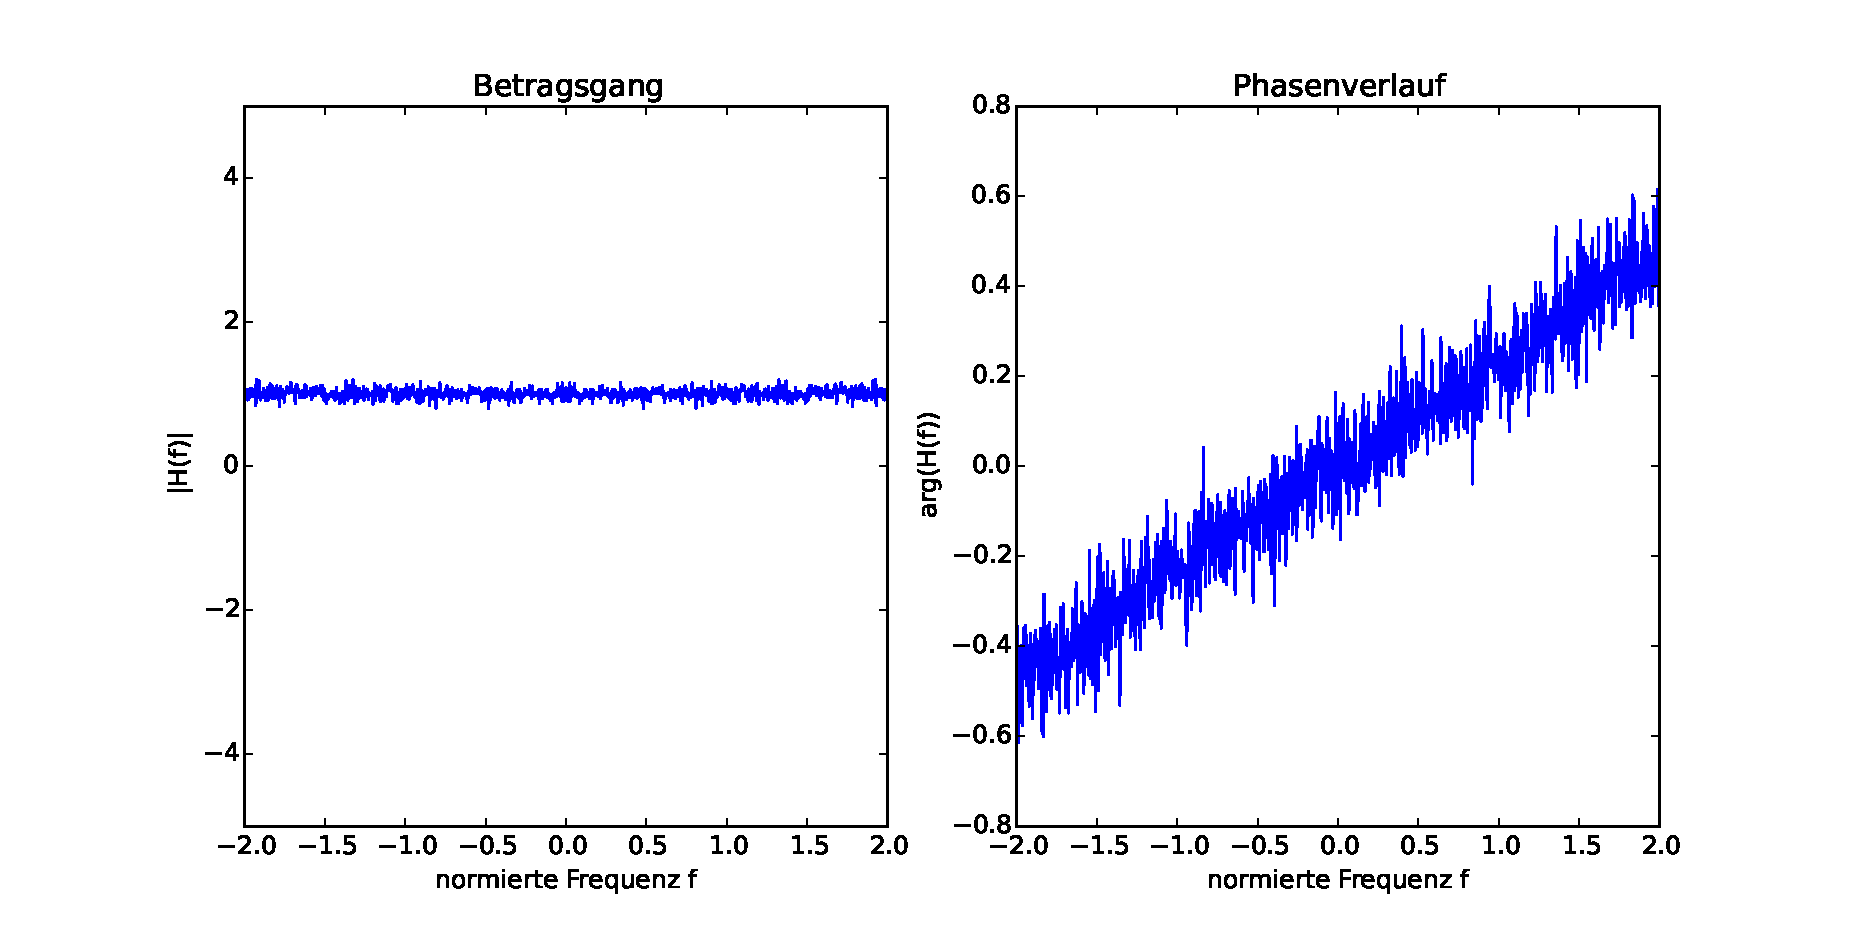
\includegraphics[width=\textwidth]{images/AWGN}
	\caption{Übertragungsverhalten eines \gls{AWGN}-Kanals}
	\label{fig: AWGN-Plot}
\end{figure}

\subsection{Mehrwegeausbreitung}
\label{chap2.2.2:Mehrwege}
Ein weiterer Störeinfluss ist die Mehrwegeausbreitung. Das Signal erreicht nicht nur über die Sichtverbindung (\gls{LOS}) das Ziel, sondern wird an Objekten in der Umgebung reflektiert und gestreut. Diese gestreuten Signalanteile überlagern sich am Empfänger mit dem \gls{LOS}-Signal additiv. Das \gls{LOS}-Signal ist dann nicht mehr klar von den Umwegpfaden trennbar. Ein solcher Kanal kann durch mehrere parallele  Verzögerungsglieder modelliert werden. Diese werden mit einem Dämpfungsfaktor $\alpha_i$ gewichtet und aufgrund der Beschaffenheit der Reflektoroberfläche zusätzlichen in der Phase gedreht, was durch einen komplexen Zeiger $\e^{j\Phi_i}$ modelliert werden kann. Je nach Anzahl $L$ und Gewichtung $\alpha_i$ der Umwegpfade, ist die Phase mehr oder weniger stark verfälscht. Für die Impulsantwort des Kanals ergibt sich daher folgender Ausdruck:

\begin{equation}
	\label{eq:Mutipath}
	h(t) = \sum_{i = 0}^L \, \alpha_i \, \delta(t - \tau_i)\, e^{j\Phi_i} \;\;\laplace\;\; H(f) =  \sum_{i = 0}^L \, \alpha_i \, e^{-j2\pi f \tau_i + \Phi_i}
\end{equation}

Um die Komplexität des Kanalmodells nicht zu groß werden zu lassen, sollen in dieser Arbeit zunächst nur Betrachtungen mit einem Umwegpfad gemacht werden.
In Abbildung \ref{fig:MehrwegeZeiger} ist veranschaulicht, wie sich die Phase zweier additiv überlagerter komplexer Zeiger verhält. Der in rot dargestellte, mit $\alpha$ skalierte Vektor des Umwegpfades dreht mindestens bis $\varphi_{LOS}$, da die Sichtverbindung der kürzest mögliche Pfad ist. 

\begin{figure}[htbp]
	\centering
	\hspace*{2cm}
	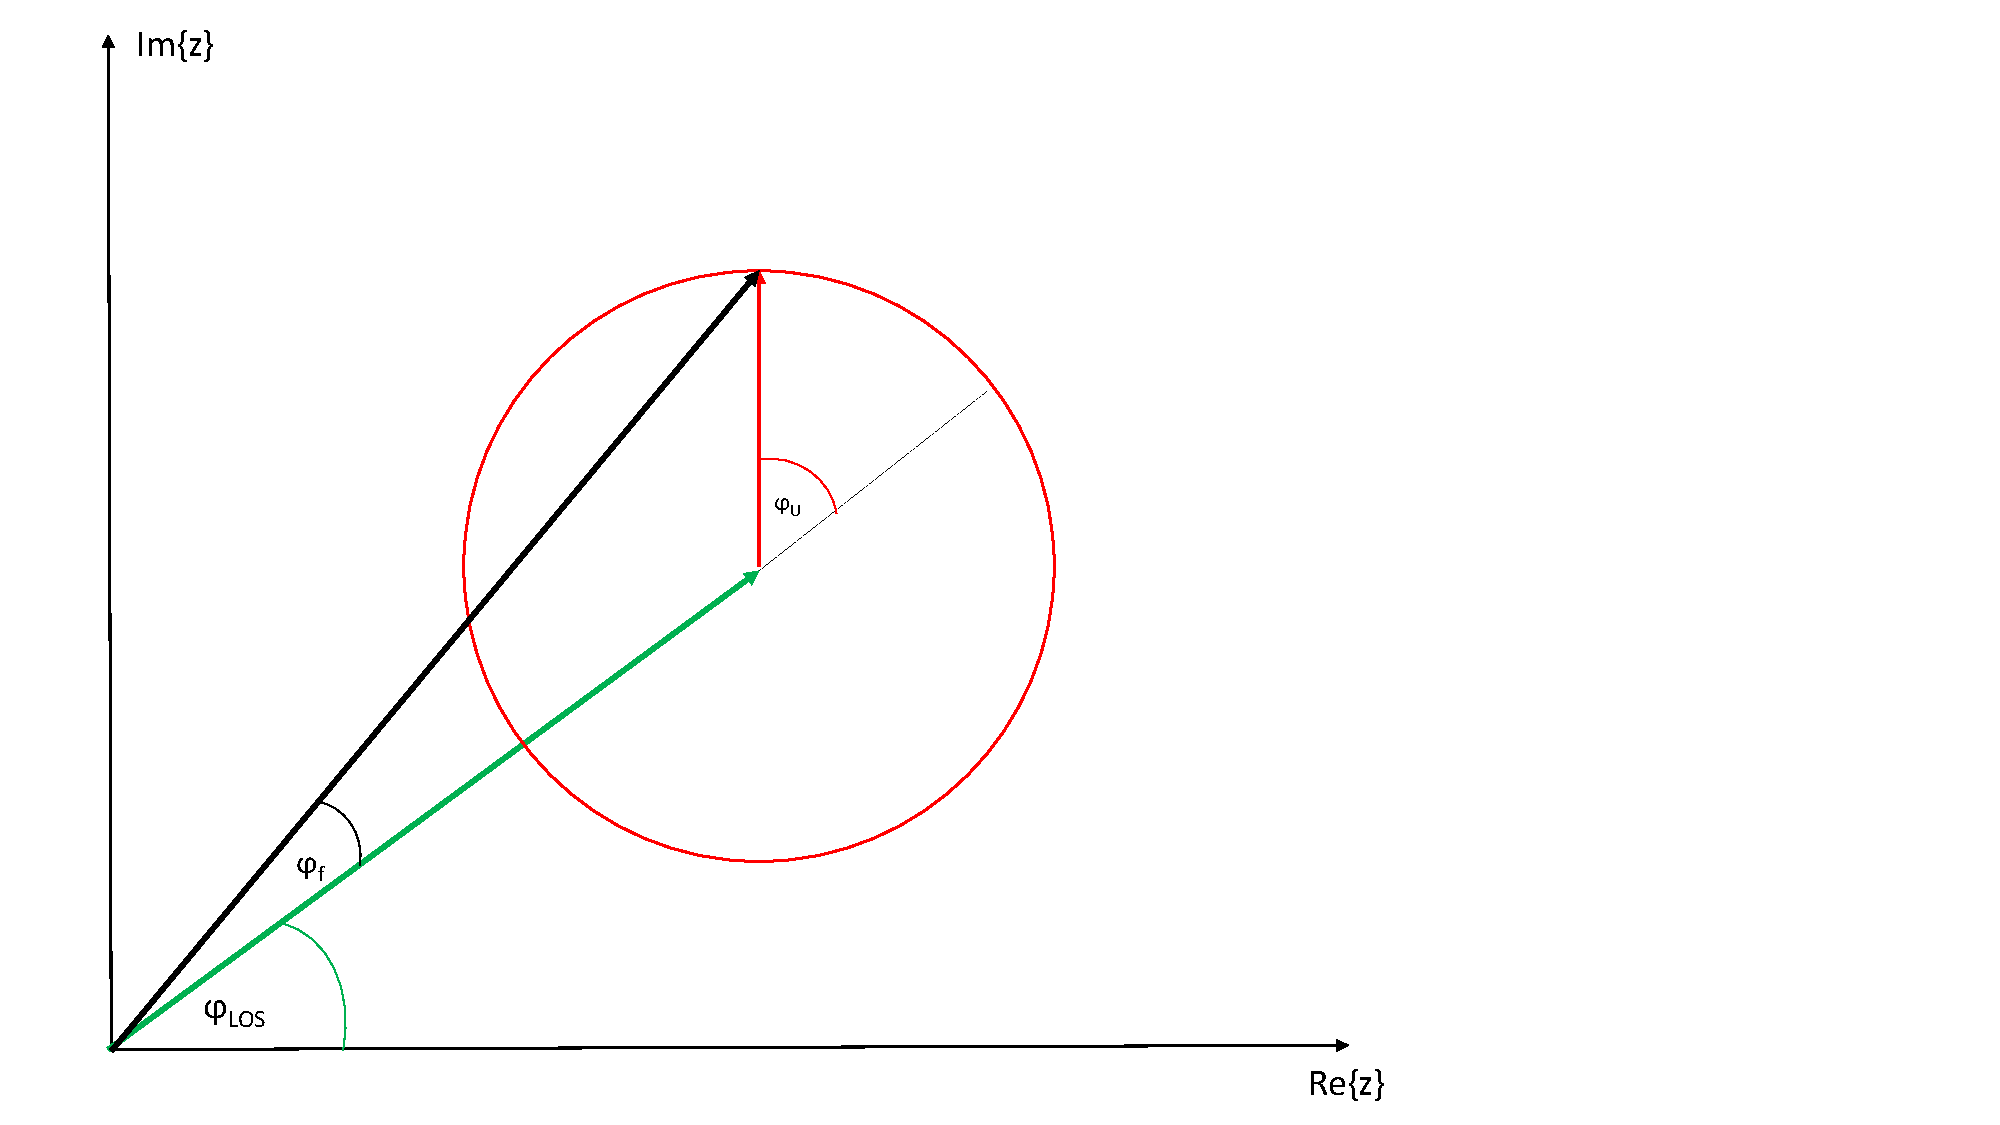
\includegraphics[width = \textwidth]{images/MehrwegZeiger}
	\caption{Zwei additiv überlagerte komplexe Zeiger}
	\label{fig:MehrwegeZeiger}
\end{figure}

Abhängig von der Länge des Umwegpfades, dreht er sich um $\varphi$\textsubscript{u} weiter. Der in der Abbildung \ref{fig:MehrwegeZeiger} schwarze, resultierende Vektor, hat nun eine, um $\varphi$\textsubscript{f} von $\varphi$\textsubscript{LOS} abweichende Phase. Wenn sämtliche Umwege betrachtet werden, dreht sich der Umwegvektor auf einem Kreis um die Spitze des LOS-Vektors. $\varphi$\textsubscript{f} schwingt dabei sinusartig um $\varphi$\textsubscript{LOS}, wobei die Amplitude dieser Schwingung von dem Skalierungsfaktor $\alpha$ abhängt. Ein Sonderfall entsteht bei $\alpha = 1$. Hier entspricht die Amplitude des Umwegpfades der des LOS-Pfades und sorgt bei einem $\varphi$\textsubscript{u} von $180^\circ$ für einen Phasensprung. In diesem Fall verhält sich $\varphi$\textsubscript{f} wie ein Sägezahn um $\varphi$\textsubscript{LOS} \cite{mehrwegeausbreitung}.


\begin{figure}[htbp]
	\centering
	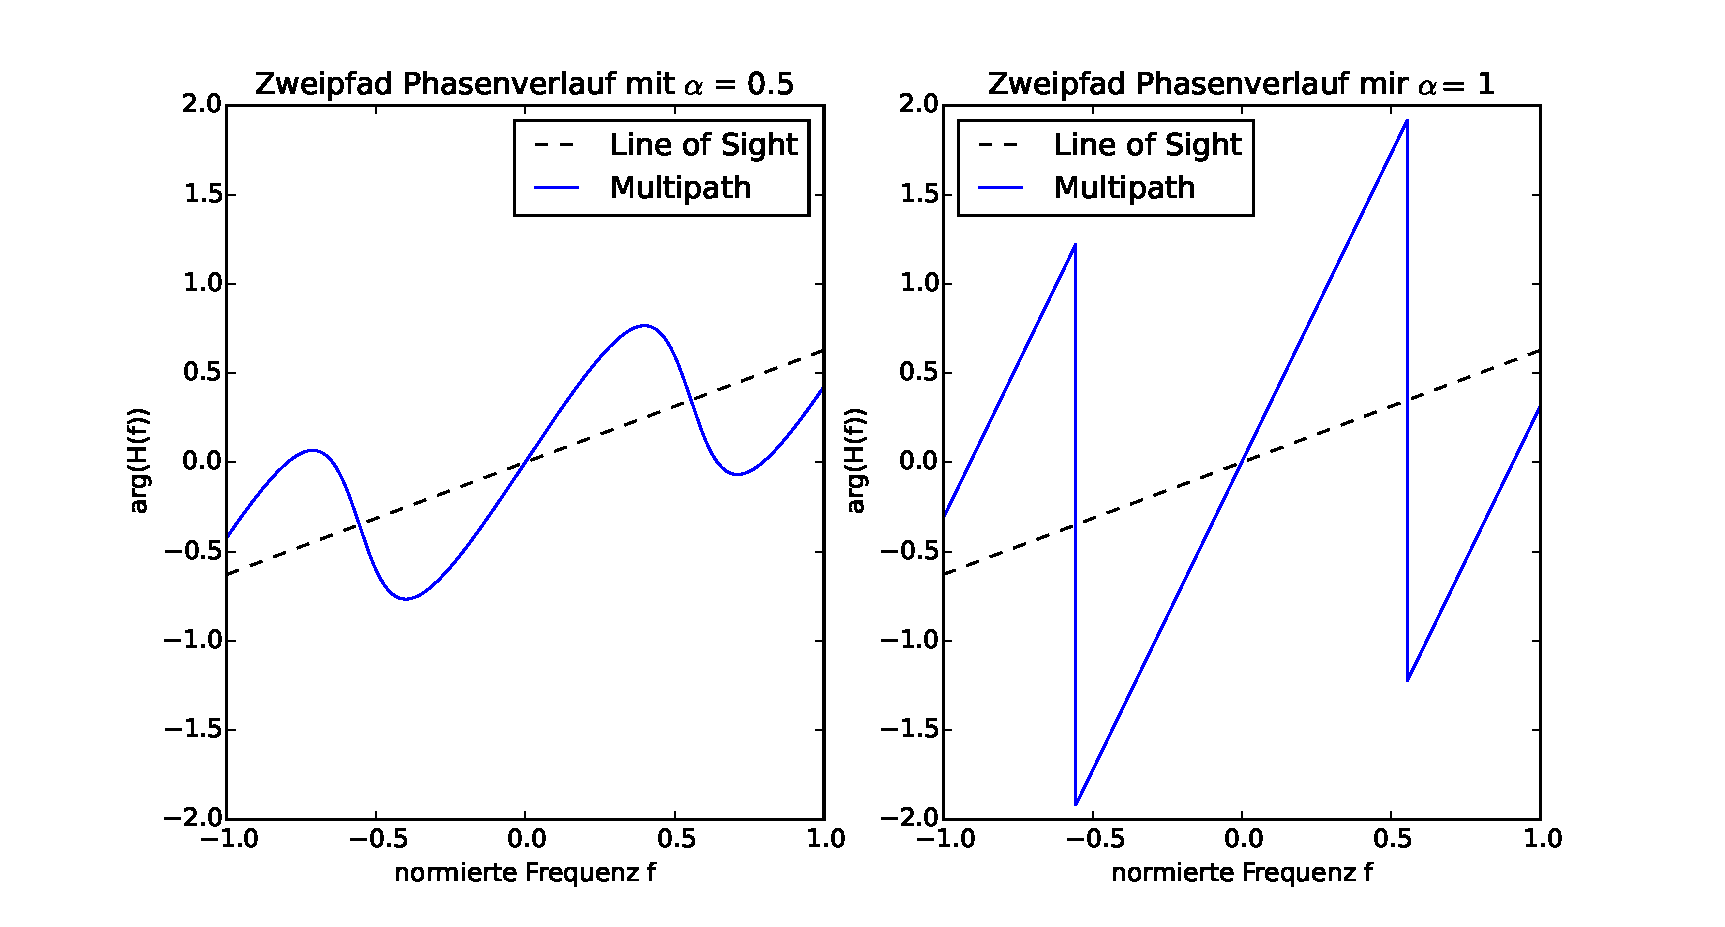
\includegraphics[width=\textwidth]{images/MutipathSim}
	\caption{Phasenverlauf eines Zweipfadkanals}
	\label{fig:MutipathSim}
\end{figure}

In Abbildung \ref{fig:MutipathSim} wurde beispielhaft ein solcher Phasenverlauf eines Zweipfadkanals simuliert. Auf der linken Seite ist die sinusförmige Schwingung um die eigentliche Phasenrampe und auf der Rechten der Sägezahn zu erkennen.
In Abbildung \ref{fig:MehrwegeZeiger} ist zu sehen, dass die Amplitude des Signals nicht unberührt vom zweiten Pfad bleibt. Teilweise trägt der Umweg konstruktiv, teilweise auch destruktiv zur Amplitude bei. Dabei kann es sogar zur völligen Auslöschung des Zeigers kommen. Dies führt bei einer Multiplikation mit dem Signal zu einer Auslöschung des Subträgers. Ein solcher Kanal wird deshalb auch frequenzselektiver Fadingkanal genannt, da, je nach Umweglänge, unterschiedliche Frequenzen stark gedämpft werden. In Abbildung \ref{fig:MutipathSim_abs} wird der Betragsgang zum obigen Phasenverlauf aufgezeigt, anhand dessen der frequenzselektive Schwund an zwei Stellen im Band erkennbar wird. In diesem Beispiel wäre die Bestimmung der Phasendifferenz nicht mehr möglich, wenn genau diese Stellen mit Subträgern belegt worden wären. All diese Eigenschaften lassen darauf schließen, dass eine geringe Anzahl von Subträgern für die Phasendifferenzbestimmung sehr anfällig für den Mehrwegekanal sind. Diese Erkenntnis gibt einen Hinweis darauf, wie Signale entworfen werden müssen, damit sie möglichst robust gegenüber den Einflüssen des Kanals sind: Je mehr Subträger das Signal hat, desto besser lässt sich der Kanal auflösen. 

\begin{figure}[htbp]
	\centering
	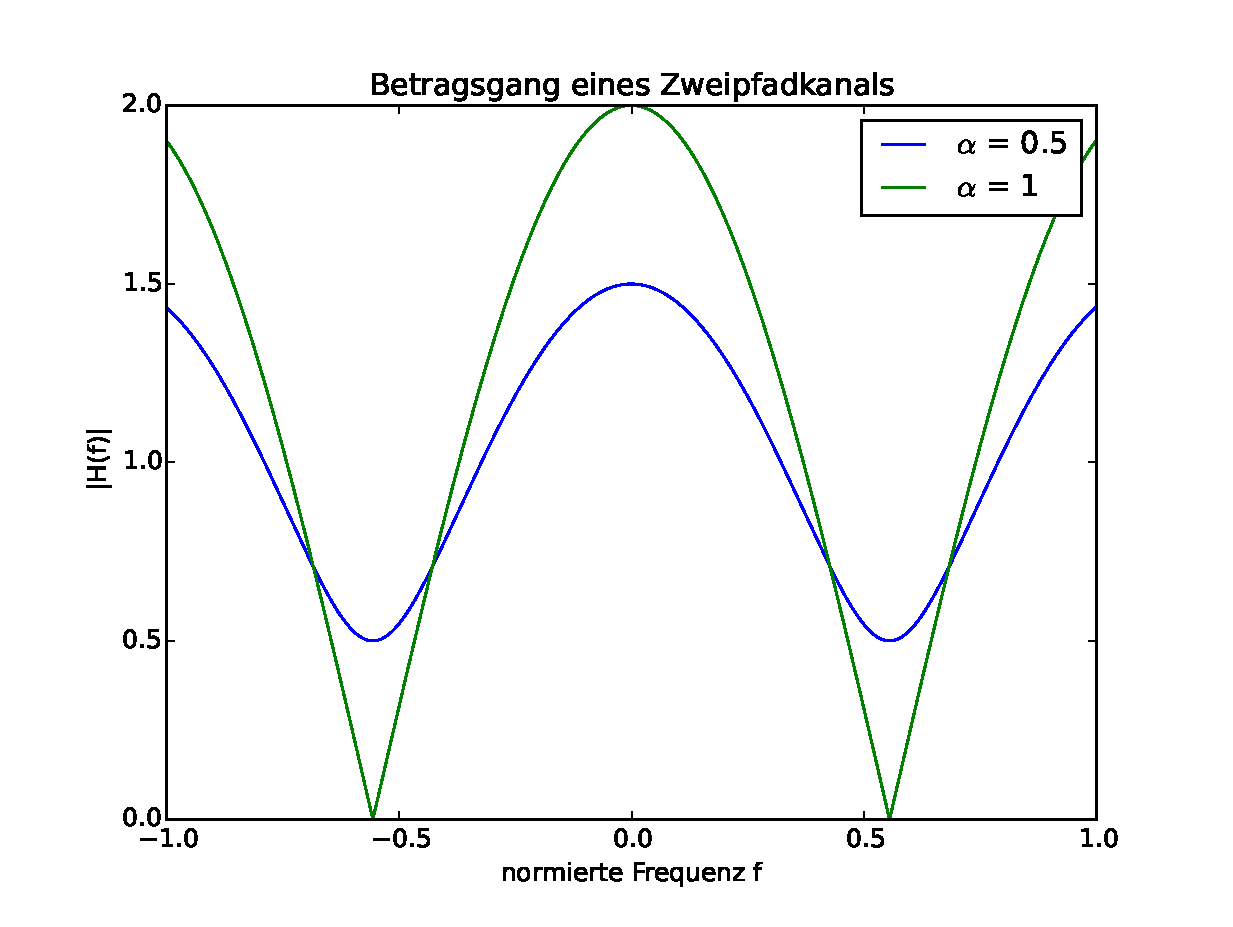
\includegraphics[scale=0.5]{images/MutipathSim_abs}
	\caption{Betragsgang eines Zweipfadkanals}
	\label{fig:MutipathSim_abs}
\end{figure}

\section{Schätztheorie}
\label{chap2.3:Schätztheorie}
Aus dem Kanalmodell wird ersichtlich, dass Signale mit einem weißen Spektrum weniger anfällig gegenüber den Einflüssen des Mehrwegekanals wären, da die Fehleinflüsse frequenzselektiv sind. Die Eigenschaften, die ein Signal benötigt, um Schätzfehler unter Einfluss eines \gls{AWGN}-Kanals zu minimieren, sind jedoch noch nicht offensichtlich. Die Schätztheorie beschäftigt sich damit, wie die Parameterschätzung bei gestörten Größen verbessert werden kann. Im Folgenden sollen einige Erkenntnisse der Schätztheorie genauer erläutert werden, um verständlich zu machen, wie ein Schätzer und das Signal aufgebaut sein müssen damit möglichst wenig Fehler verursacht werden. 

Die Aufgabe besteht darin, aus einer Reihe von Beobachtungswerten $x$ einen unbekannten Parameter $\theta$ zu schätzen. 
Um einen Schätzer zu entwerfen, muss zunächst ein mathematisches Modell, zum Beschreiben der Beobachtungswerte gefunden werden. Da diese Werte zufällig sind, werden sie durch ihre \gls{WDF} $p(x;\theta)$ beschrieben. Diese wird, durch die zu schätzende Größe $\theta$, parametrisiert. Die Funktion $p(x;\theta)$ ist zunächst unbekannt und muss aus den Gegebenheiten, z.B. dem Kanalmodell, bestimmt werden.  Bei einem \gls{AWGN}-Kanal handelt es sich um eine Gaußverteilung mit Varianz $\sigma^2$ und Mittelwert $\theta$. 

\begin{equation}
	\label{eq:gaussverteilung}
	p(x;\theta) = \frac{1}{\sqrt{2\pi\sigma^2}} \; e^{-\frac{(x-\theta)^2}{2\sigma^2}}
\end{equation}

Sobald eine solche \gls{WDF} spezifiziert wurde, besteht die Aufgabe darin einen optimalen Schätzer, und somit eine  Abbildung der Beobachtungswerte auf den jeweiligen Parameterwert, wie in \eqref{eq:Schätzabbildung} zu finden, welcher einen möglichst geringen Fehler macht. 

\begin{equation}
	\label{eq:Schätzabbildung}
	\hat{\theta} = g(x[0],x[1],x[2]...,x[N-1])
\end{equation} 

Bei jedem zu schätzenden Parameter gibt es zwei Varianten. Der eigentliche Parameterwert $\theta$, welcher unbekannt ist und der Schätzwert $\hat{\theta}$.
Da die Werte $x$ aus einer Zufallsvariablen $X$ entstanden sind, müssen die Schätzwerte $\hat{\theta}$ auch zufällig sein. Aus diesem Grund können diese nur mit statistischen Mitteln, wie Erwartungswert $E[\;]$ und Varianz $Var(\;)$, evaluiert werden. 
Schätzer können in drei Klassen eingeteilt werden:

\begin{enumerate}
	\item erwartungstreue Schätzer (unbiased estimator): $E[\hat{\theta}(X)] = \theta$
	\item Schätzer mit bekannter Ablage B (biased estimator): $E[\hat{\theta}(X)] = \theta + bias$
	\item Schätzer mit unbekannter Ablage B($\theta$):  $E[\hat{\theta}(X)] = \theta + bias(\theta)$
\end{enumerate}

 Um einen Schätzer zu optimieren, wäre der erste Gedanke den mittleren quadratischen Schätzfehler zu minimieren. Der \gls{mse} ist definiert durch 
 
\begin{equation}
	\label{eq:MSE}
	mse(\hat{\theta}) = E \left[(\hat{\theta} - \theta)^2\right] = var(\hat{\theta}) + bias^2(\theta)
\end{equation}  

Nach \cite[S.19]{kay1993fundamentals} besteht dieser aus der Varianz des Schätzwertes und der Ablage zum Quadrat. Damit man diesen Ausdruck minimieren kann, muss die Ablage bekannt sein. Diese ist allerdings vom zu schätzenden Parameter $\theta$ selbst abhängig. Deshalb ist es nur möglich einen \emph{minimum}-\gls{mse}-\emph{estimator} zu finden, wenn die Ablage bekannt ist. Dies ist meistens jedoch nicht der Fall. Wenn der Schätzer keine Ablage hat, ist es möglich die Varianz zu minimieren. Ein solcher Schätzer nennt sich dann  \gls{mvue}. Dieser Schätzer existiert nicht immer. Falls ein solcher Schätzer existiert, gibt es jedoch auch keine Methodik ihn sicher zu finden\cite[S.20f.]{kay1993fundamentals}. 

\subsection{Cramer Rao Lower Bound}
\label{chap2.3.1:CRLB}
Möglich ist es aber, eine untere Schranke für die Varianz des Fehlers zu berechnen. Eine solche Schranke ermöglicht es Schätzer mit ihr zu vergleichen. Wenn die Fehlervarianz des Schätzers auf der Schranke liegt, wurde der \gls{mvue} gefunden. Diese Schranke nennt sich \gls{CRLB} (deutsch: Cramer-Rao-Schranke). Im folgenden Kapitel wird ihre Berechnung genauer erläutert.

Ausgangspunkt ist die \gls{WDF}. Wenn diese Funktion vom Parameter $\theta$ abhängig ist und eine Wahrscheinlichkeitsdichteverteilung für den Beobachtungsvektor $x$ liefert, wird sie als Likelihood-Funktion bezeichnet. Ein Maximum-Likelihood-Schätzer wird versuchen über alle Parameter $\theta$ diese Funktion zu maximieren, um somit einen Schätzwert $\hat{\theta}$ zu finden. Wenn diese Funktion besonders steil verläuft, wie in Abbildung \ref{fig:ML_Herleitung} auf der linken Seite angedeutet, und ein eindeutiges Maximum hat, ist dessen Angabe mit geringerer Abweichung möglich. 

\begin{figure}[htbp]
	\centering
	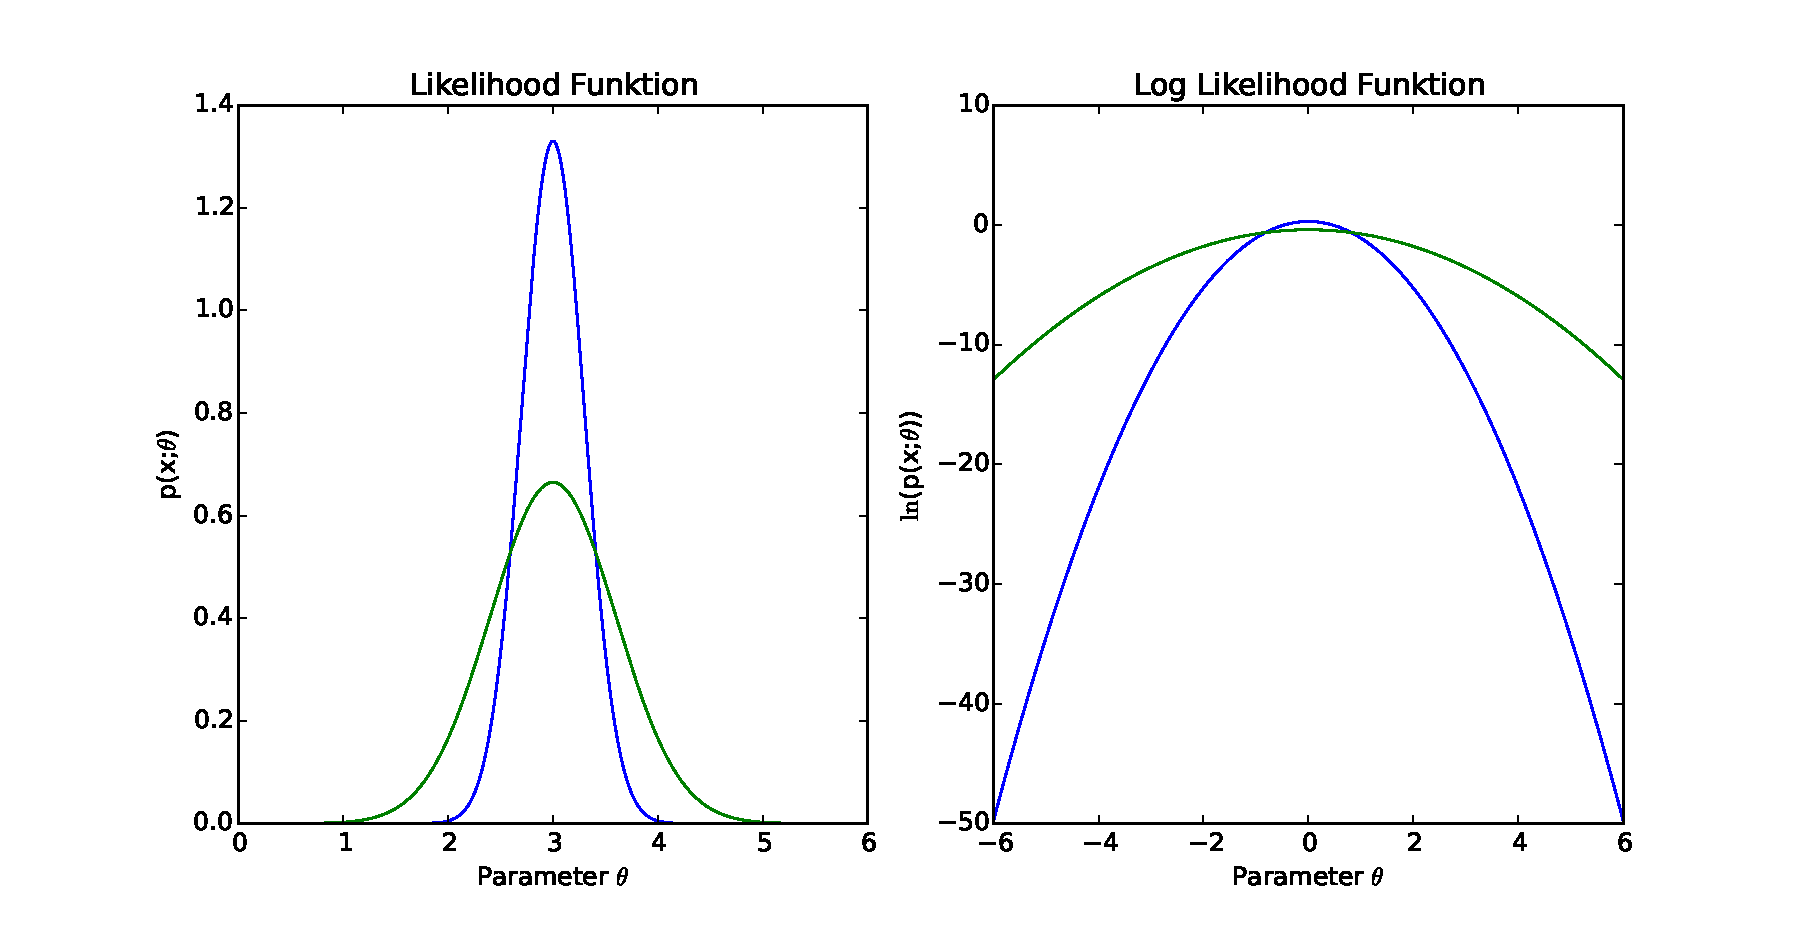
\includegraphics[width = \textwidth]{images/ML_Herleitung}
	\caption{Maximum-Likelihood- und Log-Likelihood Funktion für unterschiedliche $\sigma$}
	\label{fig:ML_Herleitung}
\end{figure}

Die blau Kurve ist eine Normalverteilung mit sehr kleiner Varianz $\sigma^2$. Da die Varianz der grünen Kurve größer ist, ist die Funktion flacher. Die Werte um das Maximum der grünen Kurve, bilden auf einen größeren Parameterbereich ab. Daher erzeugt ein verfehlen des Maximums einen größeren Parameterfehler. Wenn die Kurve steil verläuft, wie bei der Blauen, wird auf einen wesentlich kleineren Parameterbereich abgebildet. Somit hält sich der Schätzfehler, beim verfehlen des Maximums in grenzen. Das bedeutet somit auch, dass die Steilheit der Likelihood-Funktion ein Maß dafür ist, wie genau man den gesuchten Parameter schätzen kann. Diese Steilheit kann über die Krümmung der Log-Likelihood-Funktion quantifiziert werden\cite[S.29]{kay1993fundamentals}. Die Krümmung nimmt mit steigender Steilheit zu und berechnet sich nach \eqref{eq:Curvature}. 

\begin{equation}
	 \label{eq:Curvature}	
	 -E \left[\frac{\partial^2 \ln p(x;\theta)}{\partial \theta^2} \right]
\end{equation}

Aus dieser Beziehung wird ersichtlich, dass die Varianz proportional zur Inversen der Krümmung der Log-Likelihood-Funktion ist. Sie gibt die bestmögliche Genauigkeit einer Schätzung an und bildet deshalb eine untere Schranke.

\begin{equation}
	\label{CRLB}
	Var(\hat{\theta}(X)) \geq \frac{1}{- E \left[ \frac{\partial^2 \ln(p(x;\theta))}{\partial\theta^2} \right]}
\end{equation} 

Damit diese Schranke gilt, muss die WDF $p(x;\theta)$ die Regularitätsbedingungen nach \eqref{eq:refularity1} und \eqref{eq:regularity2} erfüllen.

\begin{equation}
	\label{eq:refularity1}
	E \left[\frac{\partial\ln p(x;\theta)}{\partial \theta}\right] = 0	
\end{equation}

\begin{equation}
	\label{eq:regularity2}
	\frac{\partial}{\partial \theta} \int \hat{\theta}(x) p(x;\theta)dx = \int \hat{\theta}(x)\frac{\partial p(x;\theta)}{\partial \theta} dx
\end{equation}

\subsection{CRLB für Distanzschätzung im AWGN-Kanal}
\label{chap2.3.2:CRLB für Distanzschätzung im AWGN}

In \cite[S.33]{kay1993fundamentals} ist diese Schranke für verschiedene Schätzprobleme ausgewertet worden. Unter Anderem auch für die Phasenschätzung in einem \gls{AWGN}-Kanal. Für dieses Kanalmodell wurde hergeleitet, dass kein Schätzer ohne Ablage gefunden werden kann, welcher die Schranke für alle möglichen Phasenwerte erreicht. Deshalb gilt es einen Schätzer zu suchen, der möglichst nah an die Schranke herankommt. In \citep{nowak2014system} wurde die \gls{CRLB} für Distanzschätzung in einem \gls{AWGN}-Kanal angegeben \eqref{eq:CRLB_Range}, welche in der späteren Auswertung Verwendung finden soll.

\begin{equation}
	\label{eq:CRLB_Range}
	\sigma^2_{range} \geq \frac{c_0^2}{(2\pi)^2 \cdot T_s \cdot B \cdot \frac{E}{N_0} \cdot \beta_{rms}^2}
\end{equation}

$T_s$ entspricht der Zeitdauer des Signals, $B$ der Bandbreite, $\frac{E}{N_0}$ dem Signal-zu-Rausch-Verhältnis und $\beta_{rms}^2$ der effektiven Bandbreite (rms-Bandbreite). Letzteres beschreibt die Verteilung der Signalenergie auf einem gegebenen Band und ist definiert durch \eqref{eq:effektiveBandwidth}. Die Signalenergie $E$ lässt sich nach Parseval aus dem Spektrum $S(f)$ des Signals berechnen \cite[S.30]{SignaleSysteme}.

\begin{equation}
	\label{eq:effektiveBandwidth}
	\beta^2_{rms} = \int_{-\frac{B}{2}}^\frac{B}{2} f^2 \cdot |S(f)|^2 df
\end{equation}

Da meist die Parameter Bandbreite, Zeitdauer und Signal-Rausch-Verhältnis vorgegeben sind, bietet es sich an, die Schranke über die effektive Bandbreite zu verbessern. Mit einer steigenden effektiven Bandbreite, wird die \gls{CRLB} kleiner. Da $\beta^2_{rms}$ mit der quadratischen Frequenz skaliert wird, erreicht sie ihr Maximum, wenn die gesamte Signalenergie an die Bandkanten verteilt wird.
Somit wurde eine Signaleigenschaft gefunden, welche die Schätzvarianz der Parameter eines Signales, unter Einfluss eines \gls{AWGN}-Kanals minimiert. 

\subsection{Fehlerhüllkurven für Mehrwegeausbreitung}
\label{chap2.3.3:Hüllkurven}
Den Ansatz eine untere Schranke für die Varianz zu finden, könnte auch bei Mehrwegekanälen verfolgt werden.

\begin{figure}[htbp]
	\centering
	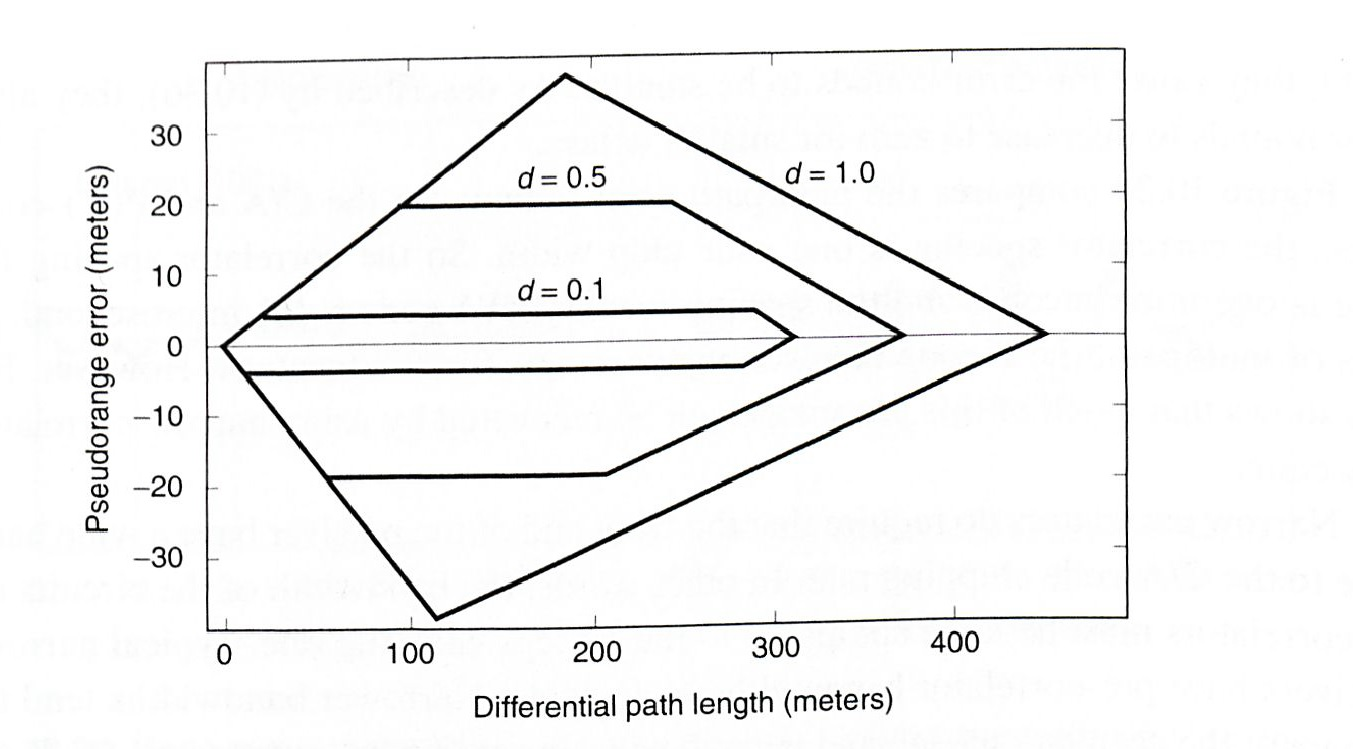
\includegraphics[scale=0.4,angle = -0.8]{images/Hullkurve}
	\caption{Mehrwege-Fehlerhüllkurve wie sie in GPS verwendet wird \cite{gps}}
	\label{fig:GPS Hüllkurve}
\end{figure}

Um die \gls{CRLB} für einen Mehrwegekanal zu berechnen, muss allerdings dessen statistisches Modell vorhanden sein. Für den Betragsgang der Übertragungsfunktion eines solchen Kanals gibt es Verteilungen, wie beispielsweise die Rayleigh-Verteilung. Diese ist allerdings nur für die Messung der Signalleistung relevant. Ist man jedoch an einer Messung der Phase interessiert, existiert bisweilen kein gutes Modell. In \cite{Lindner_CRLB} wurde die \gls{CRLB} für einen Zweipfadkanal berechnet. Bei der Arbeit geht es um Richtungsmessung, welche der Phasenmessung sehr ähnlich ist. Das Ergebnis zeigt allerdings, dass für starke Korrelation zwischen den beiden Pfaden, die \gls{CRLB} divergiert. Dies gilt sogar für hohe Dämpfungsfaktoren $\alpha$ des zweiten Pfades. Deshalb ist es nicht sinnvoll, dieses Maß für einen solchen Kanal zu verwenden. Die Schätzverfahren sollen mit einer Methode aus dem Forschungsbereich des \gls{GPS} evaluiert werden.
Bei \gls{GPS} wird die Signallaufzeit über Korrelation gemessen. Wenn der Umwegpfad kürzer als die Zeitdauer eines Samples ist, kann der Korrelator diesen nicht mehr auflösen. Diese Effekte werden mittels Fehlerhüllkurven, wie sie beispielhaft in Abbildung \ref{fig:GPS Hüllkurve} zu sehen sind, untersucht. Eine Mehrwege-Fehlerhüllkurve trägt den Laufzeitfehler über die Differenz aus Umwegpfad und LOS auf. Dabei lassen sich die Einflüsse der Länge des Umwegpfades, aber auch der Einfluss der Phasendrehung durch Reflektoren, gut veranschaulichen.
Zur Auswertung der Robustheit gegenüber Mehrwegeausbreitung sollen auch in dieser Arbeit Fehlerhüllkurven verwendet werden. 
 

\section{Signalcharakteristik}
\label{chap2.4:Signalcharakteristik}
Aus dem Kanalmodell und der Schätztheorie können einige Erkenntnisse darüber erlangt werden, wie ein Signal auszusehen hat, damit es trotz der Einflüsse des Kanals, robust gegenüber Mehrwegeausbreitung und schätzfehler-minimierend gegenüber dem \gls{AWGN}-Kanal ist. In diesem Kapitel sollen diese Eigenschaften zusammengetragen und Möglichkeiten zur Erzeugung solcher Signale vorgestellt werden. 


Da aus \eqref{eq:CRLB_Range} die Beziehung $\sigma_{range}^2 \sim \nicefrac[]{1}{\beta_{rms}^2}$ entnommen werden kann, ist es nötig die effektive Bandbreite zu maximieren. Ein Signal mit der Signalenergie an den Bandkanten würde diese Bedingung erfüllen. Allerdings ist aus dem Kanalmodell für Mehrwegeausbreitung ersichtlich geworden, dass ein Zweiton nicht besonders robust gegenüber destruktiver Interferenz ist. Dies offenbart ein Optimierungsproblem, bei welchem möglichst viel Energie an den Bandkanten, aber auch gleichzeitig auf dem Band verteilt werden muss, um gegenüber beiden Kanalmodellen robust zu sein. Deshalb sollen Mehrtonsignale mit unterschiedlichen Subträgerverteilungen untersucht werden, um herauszufinden wie diese auf den Kanal reagieren. 
Ausgehend von einem Zweiton, werden immer mehr Träger dem Band hinzugefügt. 

Zusätzlich muss der Energiebedarf beachtet werden. Signalerzeugung energiesparsam umzusetzen ist deshalb äußerst wichtig. Im Folgenden werden zwei Möglichkeiten gezeigt, wie solche Mehrtonsignale sparsam generiert werden können. 

\subsection{Hadamard-Sequenzen}
\label{chap2.4.1:Hadamard}
Hadamard-Sequenzen bieten die Möglichkeit das Band mit unterschiedlich vielen Trägern auszufüllen, je nachdem, welche Sequenz man auswählt. Die Sequenzen resultieren aus den Zeilen einer Hadamard-Matrix. Eine Hadamard-Matrix zeichnet sich dadurch aus, dass  Zeilen- und Spaltenvektoren jeweils zueinander orthogonal sind und die Einträge nur die Werte 1 und -1 annehmen können. Das Bildungsgesetz einer solchen Matrix ist ein rekursiver Algorithmus mit dem Anfangswert $H_{1x1} = 1$. Um daraus eine $2^{\nu}x\,2^{\nu}$ Matrix zu erzeugen gilt folgende Regel: 

\begin{equation}
	\label{eq:Hadamard-Matrix}
	H_{2^{\nu} x 2^{\nu}} = 
	\begin{pmatrix}
		H_{2^{\nu}} & \;\;\,H_{2^{\nu}} \\ H_{2^{\nu}} & - H_{2^{\nu}}
	\end{pmatrix}	 
\end{equation} 

Nicht alle Zeilen einer solchen Matrix spreizen das Spektrum. Die erste Zeile einer jeden Hadamard-Matrix besteht nur aus Einsen und hat daher nur einen Gleichanteil. Eine $H_{4x4}$-Matrix erzeugt vier Sequenzen. Die erste Sequenz schwingt nicht, die Zweite ist ein Einton und die Dritte und Vierte sind zwei Varianten desselben Zweitons. Für die Signalerzeugung von Mehrtonsignale werden erst Matrizen für $\nu \geq 3$ verwendet. In \eqref{eq:Hadamard-Matrix} ist eine $H_{8x8}$ beispielhaft ausgerechnet worden. 

\begin{equation}
	\label{eq:Hadamard8x8}
	H_{8 x 8} = \begin{pmatrix}
	1&1&1&1&1&1&1&1\\
	1&-1&1&-1&1&-1&1&-1\\
	1&1&-1&-1&1&1&-1&-1\\
	1&-1&-1&1&1&-1&-1&1\\
	1&1&1&1&-1&-1&-1&-1\\
	1&-1&1&-1&-1&1&-1&1\\
	1&1&-1&-1&-1&-1&1&1\\
	1&-1&-1&1&-1&1&1&-1
	\end{pmatrix}
\end{equation}

Diese Matrix liefert acht Sequenzen. In Abbildung \ref{fig:Hadamarspektren} wurde die \gls{DFT} von Signalen, bestehend aus Wiederholungen dieser Sequenzen berechnet. Die x-Achse der Abbildungen stellt eine normierte Frequenz dar, die y-Achse den normierten Betrag der \gls{DFT}. Die erste Sequenz hat ihre gesamte Energie bei der Frequenz Null. Die zweite Sequenz ist eine cosinusartige Schwingung, welche die gesamte Bandbreite ausnutzt. Des Weiteren sind die Sequenzen 3 und 4 Schwingungen, die nur die halbe Bandbreite ausnutzen. Die Sequenzen 5 und 7 bzw. 6 und 8 sind identisch. Wenn man die Sequenzen genauer betrachtet, sind sie verschobene Varianten voneinander. Eine $H_{8x8}$-Matrix liefert für unsere Zwecke somit drei Zweitöne und vier Viertöne. Um für spätere Auswertungen mehr Subträger einzufügen, werden $H_{16x16}$- und $H_{32x32}$-Matrizen verwendet. 

\begin{figure}[htbp]
	\centering
	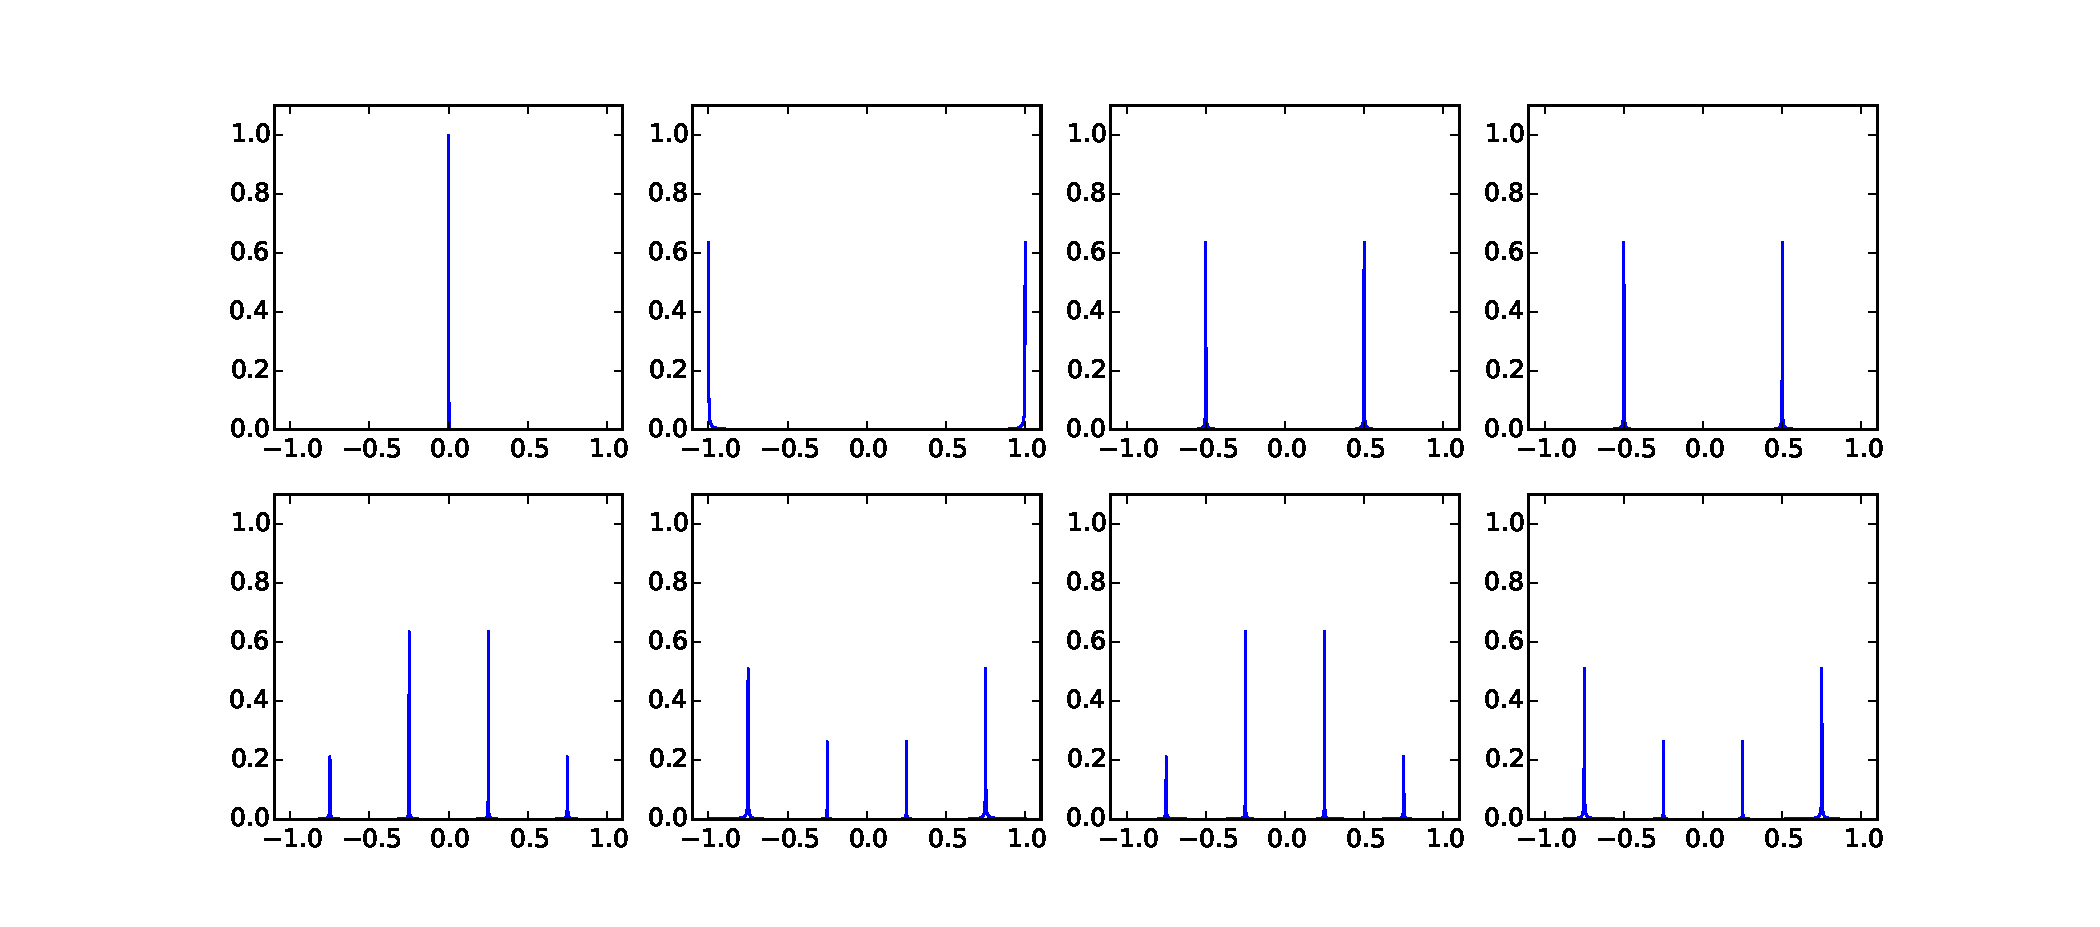
\includegraphics[width = \textwidth]{images/Hadamardspektren}
	\caption{DFT aller Hadamard-Sequenzen einer 8x8 Matrix}
	\label{fig:Hadamarspektren}
\end{figure}

Hadamard-Sequenzen können nur Spektren erzeugen, die eine gerade Anzahl an Subträgern haben und symmetrisch sind. 

\subsection{$m$-Sequenzen}
\label{chap2.4.2:m}
Eine weitere Methode zur spektralen Spreizung bieten \emph{maximal length linear shift} Register. Sie erzeugen die nach ihnen benannten $m$-Sequenzen. Eine solche Sequenz wird aus einem Schieberegister mit n Speicherzellen generiert. Die Anzahl der möglichen Zustände beträgt $2^n$. Der Zustand, bestehend aus ausschließlich Einsen, würde sich immer wieder selbst erzeugen. Ohne diesen Zustand nimmt ein Schieberegister mit $n$ Speicherzellen $2^n - 1$ Zustände ein, bevor sich die Sequenz wiederholt. Bei einem Register der Länge $n = 3$ erhält man eine Sequenz der Länge $2^3 - 1 = 7$. In Abbildung \ref{fig:Schieberegister} ist ein solches Schieberegister mit dem Anfangszustand <-1,1,1> abgebildet.  

\begin{figure}[htbp]
	\centering
	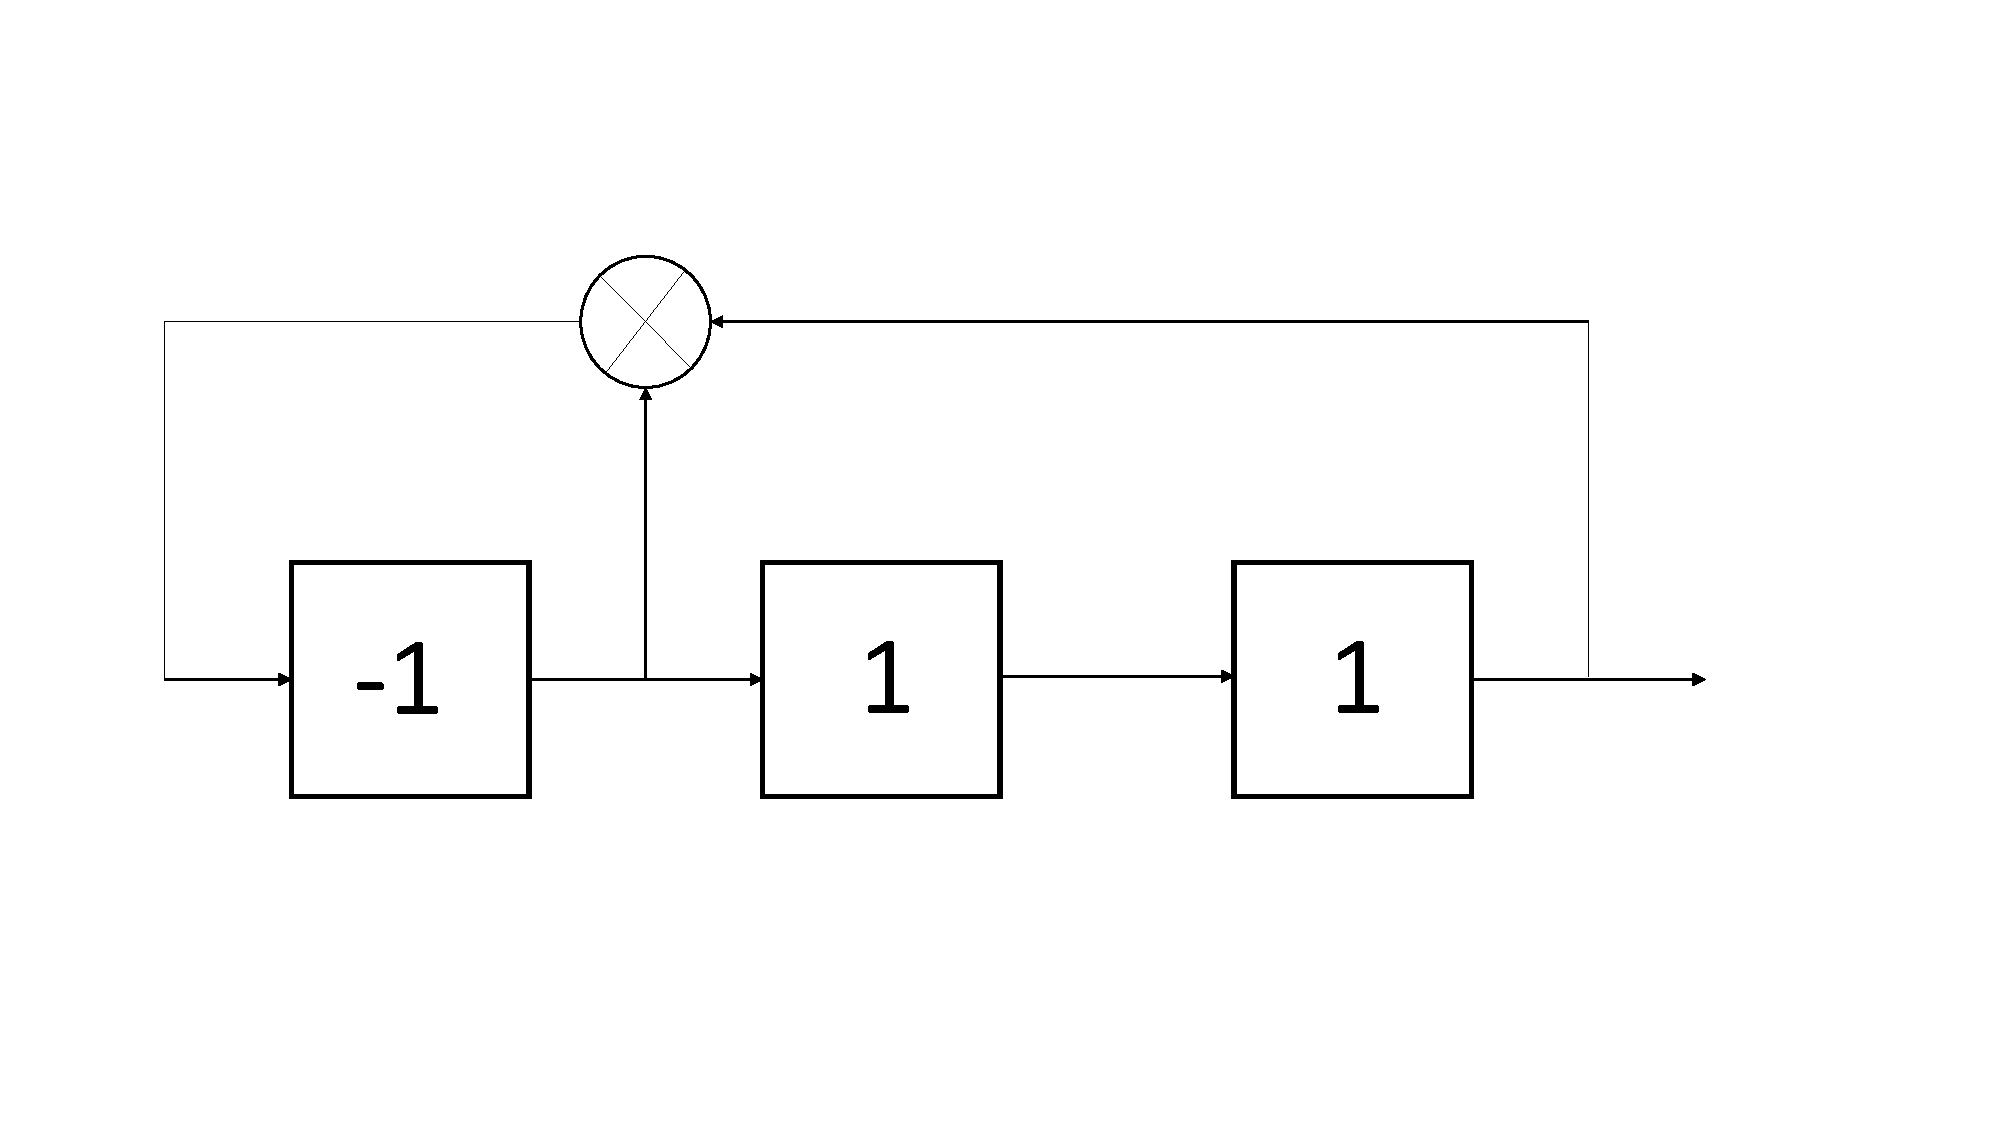
\includegraphics[width = 0.5\textwidth]{images/Schieberegister}
	\caption{Schieberegister mit Anfangszustand <-1,1,1>}
	\label{fig:Schieberegister}

\end{figure} 

Die Speicherzelle, nach der zurück gekoppelt wird, ist frei wählbar. Des Weiteren kann an mehreren Stellen zurück gekoppelt werden. Mit der Konfiguration des Registers in Abbildung \ref{fig:Schieberegister} würde demnach die Sequenz <1, 1, -1, 1, -1, -1, -1> entstehen. 
Jede $m$-Sequenz hat ein nahezu weißes Spektrum. Wird diese Sequenz periodisch wiederholt, entsteht ein Linienspektrum. Im Bereich der \gls{DFT} werden zwischen den diskreten Subträgern Nullen eingefügt. Damit entspricht die Anzahl der Subträger einer $m$-Sequenz, ihrer Länge.
